\section{Ising Model for $N>2\times 2$}
\label{sec:IsingModelNgreater}
The c++ code given in \fxnote{sec ref} is customized for the two dimensional case with $2$ spins in each of the two dimensions. 
To be able to find the expectation value of the energy and magnetization and the specific heat and susceptibility of a larger spin system, the code presented in \fxnote{secref} must be modified.

The first modification appear when introducing periodic boundary conditions to a lattice in which some elements are boundary elements while other elements are not. 
When a non-boundary element $k$ is flipped, the change in energy will be two times the energy calculated by \matref{eq:EnergyMagnetization} with $k$ being the flipped element, and $l$'s being the four neighbours of that element. 
However, a boundary element will only have two or three neighbours. 
Consider the $4\times 4$ case in \figref{fig:BoundaryConditionExample} in which the boundary element in the upper leftmost corner is flipped.  
\begin{figure}[H]
	\centering
	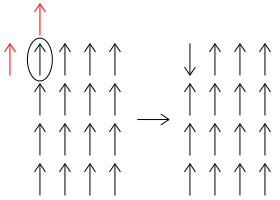
\includegraphics[width=0.3\textwidth]{Figures/BoundaryConditions.png}
	\caption{Awesome caption.}
	\label{fig:BoundaryConditionExample}
\end{figure}   
When this corner element is flipped, the change in energy will depend on the two neighbours of that element \textit{and} the last element in the same row as the flipped spin and the last element in the same column as the flipped spin due to the periodic boundary conditions.
Hence, instead of calculating the change in energy using the four if-tests in \fxnote{ref to sec}, the energy change due to a spin flip at a random entrance (x[i],y[i]) of the spin matrix is computed as in the following lines of code.
\begin{lstlisting}
DE = 2*spin_matrix(x[i],y[i])
	*(spin_matrix(x[i],periodic(y[i],-1,n)) + spin_matrix(x[i],periodic(y[i],1,n))
	+ spin_matrix(periodic(x[i],-1,n),y[i]) + spin_matrix(periodic(x[i],1,n),y[i]))
\end{lstlisting}
The periodic function in the above c++ lines takes care of the periodic boundary condition. 
Consider the source code for the function \textit{periodic}:
\begin{lstlisting}
int periodic(int entrance, int pm, int spins)
//Takes care of the periodic boundary condition of lattice with "spins" number of spins in each direction
//pm = -1 returns the "entrance" to the left of the considered element, if the considered element is not a boundary element in the first row/column of the matrix. 
//pm = 1 returns the "entrance" to the right of the considered element, if the considered element is not a boundary element in last row/column of the matrix. 
{
    return (entrance + pm + spins) % spins; // "sum mod spins"
}
\end{lstlisting}
For a non-boundary element, the element 
\text{spin-matrix(x[i],periodic(y[i],-1,n))} will be the element to the left of the chosen element 
\text{(x[i],y[i])} in the spin matrix since 
$0 < y[i] < spins$ which means that the returned spin matrix element is 
\text{spin-matrix(x[i],y[i]-1)}. 
If instead \text{(x[i],y[i])} is a boundary element, say in the upper leftmost corner as in \figref{fig:BoundaryConditionExample}, the returned element when calling the periodic function as before is then \text{spin-matrix(x[i],spins-1)}, which is the last element in the same row as the considered element, as wanted. 

Since the the only contributors to the change in energy when just one spin is flipped is the flipped spin itself and the four neighbouring spins, there are only 5 possible changes in energy for one spin flip. These are
\begin{align}
	\Delta \tilde{E} = \frac{\Delta E}{J} = \{ -8 , -4 , 0 , 4 , 8 \}
\end{align}
This means that the probability function $w(E_i) = e^{-\beta E_i}$ for accepting the move can be precalculated before the actual Monte Carlo \fxnote{right?} cycles, and the computational time is decreased. 
The inclusion of this is seen in the source code below.
\begin{lstlisting}
double w[microstates];
for (int i =0; i < microstates; i++){
    w[i] = 0;
}
for (int dE = -8; dE <= 8; dE+=4){
    w[dE+8] = exp(-dE/T);
}
for (int cycles = 1; cycles <= mccycles; cycles++){
    for (int i=0; i<n*n; i++){
    //computing row x[i] and column y[i] number as a random integer between 0 and n-1 (almost uniformly distributed)
    x[i] = (n-0.000001)*((double) rand() / (RAND_MAX));  
    y[i] = (n-0.000001)*((double) rand() / (RAND_MAX));
    DE = ....;
    if (w[DE+8] >= ((double) rand() / (RAND_MAX)))
    //comparing prop function to uniformly distributed random number between 0 and 1
    {
        spin_matrix(x[i],y[i]) = -spin_matrix(x[i],y[i]);
        E += DE;
        M += 2*spin_matrix(x[i],y[i]);
    }
    }
}
\end{lstlisting}
For the $2\times 2$ case, the probability function is then computed as the vector
\begin{align}
	\v{w} = \{e^{8/T}, 0, 0, 0, e^{4/T}, 0, 0, 0, 1, 0, 0, 0, e^{-4/T}, 0, 0, 0, e^{-8/T} \}
\end{align}
The value of $e^{8/T}$, $e^{4/T}$ and $1$ will \textit{always} be larger than or equal to the generated random number between $0$ and $1$, and hence the suggested flip will always be accepted if the flip gives rise to an energy change of $-8$, $-4$ or $0$. 
If the energy is positive, the flip will be accepted with a probability that depends on the temperature $T$. 
Higher temperature leads to more accepted moves.

Apart from the periodic function and the probability function, the way of calculating the wished quantities using this generalized c++ code is similar to the way given in \fxnote{secref}, and that the two codes give the same results for the $2\times 2$ case can be seen in \fxnote{secref, and write section with this test!}.   